% Part: sets-functions-relations
% Chapter: relations
% Section: trees

\documentclass[../../../include/open-logic-section]{subfiles}

\begin{document}

\olfileid[pt]{sfr}{rel}{tre}
\olsection{Árvores}

Um tipo particular de ordem parcial que desempenha um papel importante em
todas as partes da lógica é uma \emph{árvore}. Árvores finitas aparecem em partes
elementares da lógica: por exemplo, !!{formula}s podem ser entendidas em termos
de sua decomposição em uma árvore sintática, enquanto !!{derivation}s em
muitos sistemas de !!{derivation} também tomam a forma de árvores finitas.
%
Árvores infinitas aparecem já na prova dos teoremas de completude
para a lógica proposicional e de primeira ordem, e são usadas
em toda a lógica matemática.

O conceito de árvore da teoria dos conjuntos está intimamente relacionado à noção
de árvore na teoria dos grafos. Aqui está uma figura de uma árvore (finita):

\begin{center}
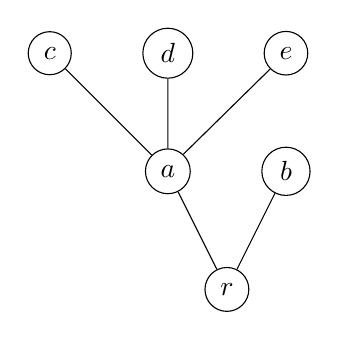
\begin{tikzpicture}[nodes={draw, circle}, -]
\node{$r$} [grow'=up]
    child { node {$a$} 
        child { node {$c$} }
        child { node {$d$} }
        child { node {$e$} }
    }
    child { node {$b$} };
\end{tikzpicture}
\end{center}

O nó mais baixo~$r$ é a raiz. Todo nó diferente de $r$ tem
exatamente um nó pai imediatamente abaixo dele. Podemos pensar na relação
em que um nó~$x$ está para um nó~$y$ se $y$ pode ser alcançado a partir de~$x$
seguindo arestas para cima como $x$ sendo um \emph{ancestral} de~$y$.

A relação de ancestralidade em uma árvore é uma ordem parcial estrita. Isso
motiva a definição teórico-conjuntista. Para enunciá-la, precisamos de dois
conceitos. Um \emph{menor elemento} em um conjunto~$A$ parcialmente ordenado
por~$\le$ é !!a{element} $x \in A$ tal que para todo $y \in A$ temos
que~$x \le y$. Um conjunto é \emph{bem ordenado} por~$\le$ se cada um de
seus subconjuntos não vazios tem um menor elemento.

\begin{defn}[Árvore]
Uma \emph{árvore} é um par $T = \tuple{A, \le}$ tal que $A$ é um conjunto
e $\le$ é uma ordem parcial em~$A$ com um único menor elemento
$r \in A$ (chamado de \emph{raiz}) tal que para todo $x \in A$,
o conjunto $\Setabs{y}{y \le x}$ é bem ordenado por~$\le$.
\end{defn}

\begin{defn}[Sucessores]
Suponha $T = \tuple{A, \le}$ é uma árvore.
Se $x,y \in A$, $x < y$, e não existe $z \in A$ tal que
$x < z < y$, então dizemos que $y$ é um \emph{sucessor} de~$x$.
\end{defn}

Os sucessores de $x \in A$ também são chamados de seus \emph{filhos}. Se
$y$ é um sucessor de~$x$, então chamamos $x$ de \emph{predecessor} ou
\emph{pai} de~$y$.

\begin{prop}
Se $\tuple{A,\le}$ é uma árvore, então todo $x \in A$ diferente da raiz
tem no máximo um predecessor.
\end{prop}

\begin{proof}
  Suponha $y_1 < x$ e $y_2 < x$ e $y_1 \neq y_2$. Então $\{y_1,
  y_2\} \subseteq \Setabs{z}{z<x}$. Como $\Setabs{z}{z<x}$ é
  bem ordenado por~$\le$, seu subconjunto $\{y_1, y_2\}$ tem um menor
  elemento, que obviamente deve ser ou $y_1$ ou~$y_2$. Então ou
  $y_1 \le y_2$ ou $y_2 \le y_1$. Supusemos que $y_1 \neq y_2$, então
  na verdade ou $y_1 < y_2$ ou $y_2 < y_1$. Como supusemos que
  $y_1 < x$ e $y_2 < x$, temos ainda que ou $y_1 < y_2
  < x$ ou $y_2 < y_1 < x$. Então $y_1$ e $y_2$ não podem ambos ser
  predecessores de~$x$.
\end{proof}

\begin{defn}
Uma árvore $T = \tuple{A, \le}$ é dita \emph{infinita} se $A$ é um
conjunto infinito, e \emph{finita} caso contrário. Se $T$ é tal que todo
$x \in A$ tem apenas um número finito de sucessores, então dizemos que $T$ é
\emph{finitamente ramificada}.
\end{defn}

\begin{defn}[Ramos]
Dada uma árvore $T = \tuple{A, \le}$, um \emph{ramo} de~$T$ é uma
cadeia maximal em~$T$, isto é, um conjunto $B \subseteq A$ tal que
para quaisquer $x, y \in B$ ou $x \le y$ ou $y \le x$, e para qualquer
$z \in X \setminus B$ existe $u \in B$ tal que nem
$z \le u$ nem $u \le z$.
%
Usamos $[T]$ para denotar o conjunto de todos os ramos de $T$.
\end{defn}

\begin{ex}
Um exemplo clássico de árvore finitamente ramificada é a
\emph{árvore binária infinita} de sequências finitas de $0$s e~$1$s,
às vezes denotada $\{0,1\}^*$ ou~$\Bin^*$, ordenada pela relação de
extensão $\sqsubseteq$ (p.ex., $101 \sqsubseteq 101101$).
Como qualquer cadeia binária pode sempre ser estendida adicionando
um $0$ ou um $1$ no final, esta árvore contém infinitos
elementos: todo elemento~$s$ tem exatamente dois sucessores, $s0$ e~$s1$. Sua raiz é a sequência vazia $\emptyseq$.
\end{ex}

\begin{ex}
De maneira um pouco mais geral, o conjunto de sequências finitas de números naturais~$\Nat^*$ com a relação de extensão~$\sqsubseteq$ também é uma
árvore. É obviamente não finitamente ramificada: todo $s \in \Nat^*$ tem
infinitos sucessores~$sn$, um para cada $n \in \Nat$. Todo $A
\subseteq \Nat^*$ que é fechado sob~$\sqsubseteq$ é uma
\emph{subárvore} de~$\Nat^*$. (Isto é, $A$ é tal que se $s \in A$
e $s' \sqsubseteq s$, então também $s' \in A$.) Todas as árvores finitas podem ser
representadas como subárvores finitas de~$\Nat^*$.
\end{ex}

\begin{prop}[Lema de K\H{o}nig]
Se $T = \tuple{A,\le}$ é uma árvore infinita finitamente ramificada,
então $T$ tem um ramo infinito.
\end{prop}

Um caso especial do Lema de K\H{o}nig amplamente usado em teoria da
computabilidade, conhecido como \emph{Lema Fraco de K\H{o}nig}, é o seguinte: qualquer
subárvore infinita de $\{0,1\}^*$ tem um ramo infinito.

\end{document}
